\documentclass[a4paper, 10pt]{article}

% Encoding
\usepackage[T1]{fontenc}
\usepackage[utf8]{inputenc}
\usepackage[english]{babel}

% Margins
\usepackage[left=2.5cm, right=2.5cm]{geometry}

% Mathematics
\usepackage{amsmath, amssymb, mathtools, amsthm}
\usepackage{xcolor}

% Bibliography (uncomment if needed)
%\usepackage{csquotes}
%\usepackage[backend=biber, sorting=none, style=nature]{biblatex}
%\addbibresource{biblio.bib}

% Personal taste
\usepackage[font=footnotesize]{caption}
\usepackage[parfill]{parskip}


\title{ans-ref-1}
\author{}

\newcommand{\red}[1]{{\color{red}#1}}

\begin{document}

\maketitle
\emph{
  page 4 line 7: I don’t understand the idea behind RandomNet: are the pixel
  values of the four filters learned by the Neural Network or randomly generated
  and fixed once for all? In the later case, the pixel values of the filters can
  not really be counted as parameters of the model. But perhaps I do not
  understand the scheme of the modification of LeNet 5 (see last comment below).
  Please explain.
}

We thank the reviewer for the interest in the matter. To clarify, we proceed as
follows: 
\begin{enumerate}
  \item we start by considering the native architecture of LeNet 5, composed of
    $60806$ trainable parameters. The first convolutional layer of LeNet
    5, in particular, takes has input feature number of $1$ and output feature
    number of $6$ (total of $156$ parameters);
  \item BorderNet: we add, before the first convolutional layer of LeNet 5,
    another convolutional layer, composed of the 4 non-trainable, oriented
    filters, shown in Fig. 2 in the paper (as a consequence, $n$ input features
    is $1$ and $n$ output features is $4$). This implies that now LeNet's first
    convolutional layer is receiving $4$ input features, and now contains $606$ 
    trainable parameters, roughly four times the number present its native
    version. In total, BorderNet contains $61256$ parameters;
  \item RandomNet: we proceed as we did for BorderNet, the only difference being
    that the added convolutional layer contains filters with \emph{random}
    non-trainable weights. Exactly as before, the underlying LeNet's first
    convolutional layer now contains $606$ trainable parameters, and RandomNet
    contains $61256$ trainable parameters.
\end{enumerate}
As (we hope) can be seen, the very addition of (trainable or non-trainable)
filters in front of LeNet 5, induces an increase in the LeNet's trainable
parameters due to the increase in input channels (from $1$ to the number of 
output filters of the added layer). Therefore, to separate the gain in
performance originating from our filters' geometry from the one arising from 
the simple increase in trainable parameter number, we compare the final accuracy
of BorderNet against RandomNet (and not LeNet 5).


\begin{figure}
  \centering
  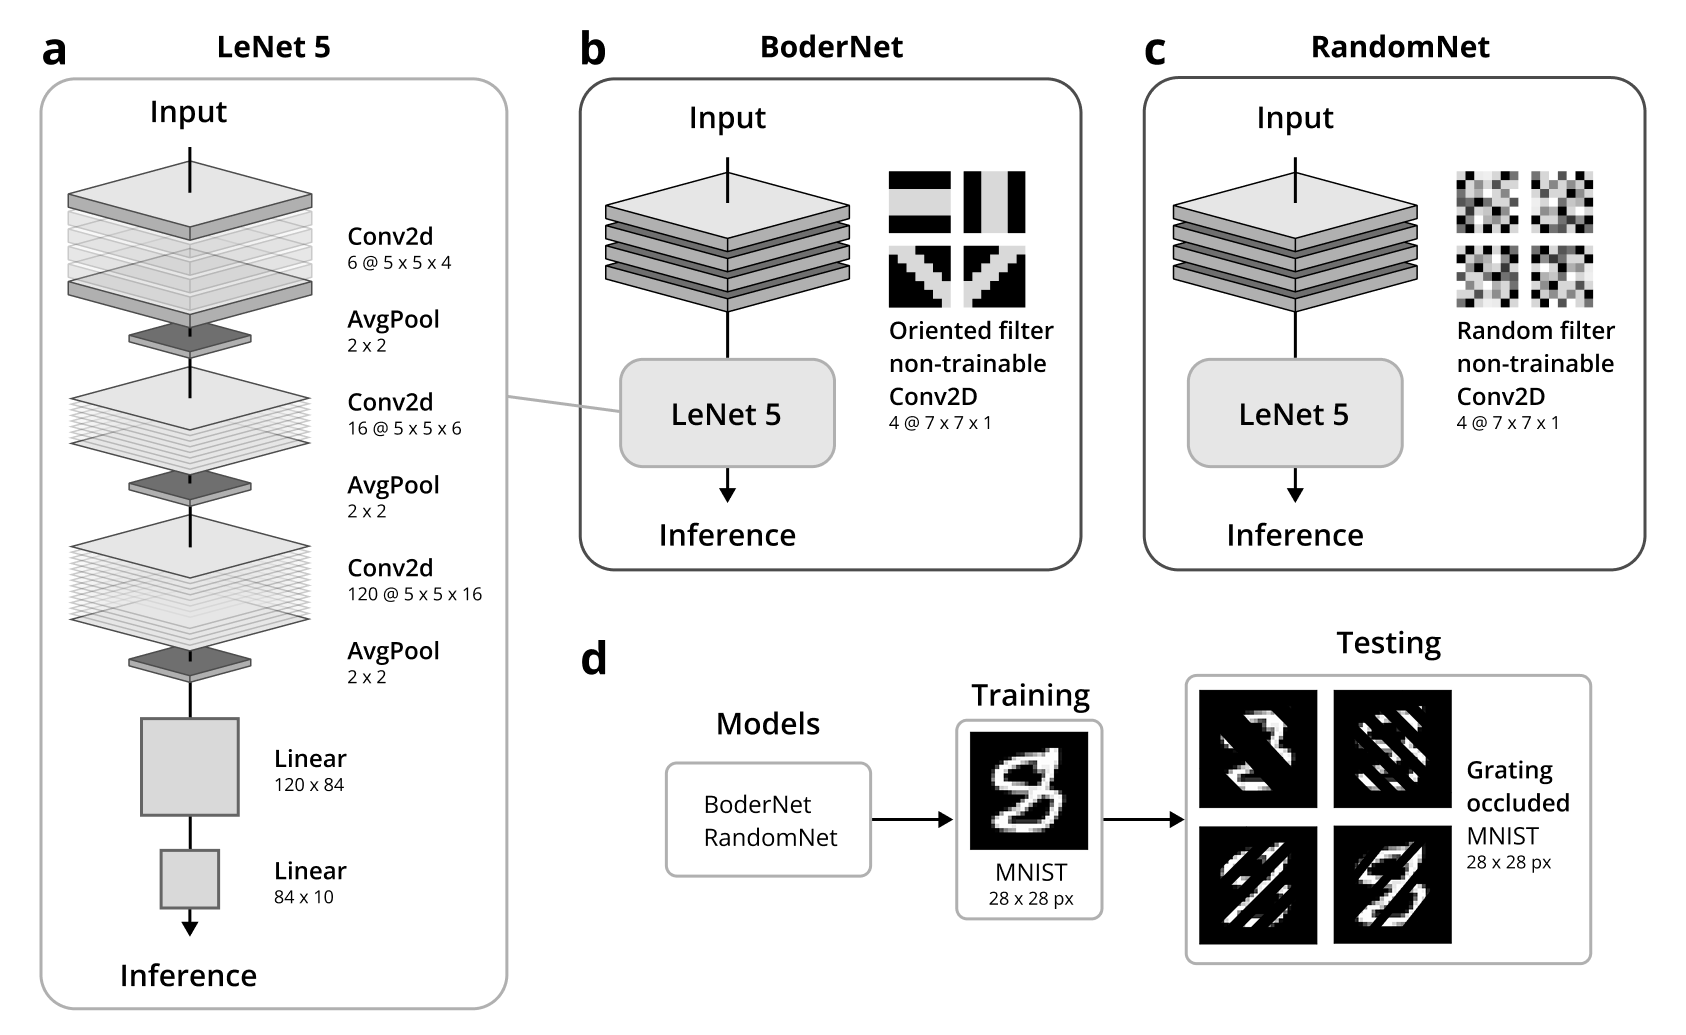
\includegraphics[width=\textwidth]{methods-bnw.png}
  \caption{
    \textbf{Outline of the papaper's model and experimental methods |} \textbf{a}
    Native structure of the LeNet 5 model (60806 trainable parameters) \textbf{b}
    BorderNet model, where an additional, non-trainable \texttt{Conv2d} layer
    composed of oriented filters is inserted ahead of the LeNet 5 structure
    (61256 trainable parameters). 
    \textbf{c} RandomNet model, differing from BorderNet only by the weights of
    the first \texttt{Conv2d} layer (random instead of oriented, 61256 trainable
    parameters). \textbf{d} Outline of the experimental procedure: training is
    conducted on the native MNIST dataset, while testing is performed after
    occlusion with different types of oriented gratings.
  }
\end{figure}
% \printbibliography

\end{document}
